\documentclass[a4paper, 12pt]{article}

\usepackage[utf8]{inputenc} % for UTF-8 support
\usepackage{graphicx}       % for images
\usepackage{hyperref}       % for hyperlinks
\usepackage{biblatex}       % for references

\bibliography{references}   % put citations here
\graphicspath{{./images/} } % put images in here

\title{AI for IMGD Final Project Report}
\author{Cole Granof \and Joe Petitti \and Matt Puentes}
\date{\today}

\begin{document}

\maketitle

\section{What We Did}

For the final AI for IMGD project we created a procedurally generated, top-down,
twin stick shooter game, called \textbf{Proc Cave Game}, inspired by games like
\textit{The Binding of Isaac} and \textit{Nuclear Throne}. In the game, the
player controls a small eyeball-like character that can move around the game
world, a large series of caves. There are several types of enemies that inhabit
the caves, including some that chase the player, others that wander around
randomly, and even some that can shoot bullets. Players fight these enemies
while exploring the cave to track down three Boss enemies, which must be
defeated to win. They can also find power-ups hidden the caves, powerful
artifacts that increase the player's abilities in unique ways.

The hero is controlled with a keyboard or gamepad, and can move around and shoot
in any direction. Like all game entities in our custom engine, the hero has a
velocity, acceleration, and drag. This allows it realistically reach a maximum
speed in a way that is simple to program and maintain.

There are three main enemy types: Chase, Scatter, and Shooter. Chase enemies
sleep until the player comes close or shoots at them, but chase after the hero
as soon as they wake up. Scatter enemies wander around the board in random and
unpredictable ways. Shooter enemies maintain their distance and fire slow-moving
projectiles at the hero. Each enemy has a random chance to be bigger. Bigger
enemies split into several smaller enemies when they are killed, providing
varying levels of difficulty.

Each enemy type has a different type of face, which is further modified by
randomly generated parameters. For example, Chase enemies have one large eye in
the center of their face, but the size and positioning of their eye and mouth is
tweaked by parameters. The game world has randomly generated color scheme, which
is applied to the cave environment as well as enemies.

The game also features a robust power-up system. All power-ups are applicable to
both the hero and the enemies---both are abstracted to a Creature superclass.
All Creatures share functionality such as speed, shot rate, and bullet damage.
In this way, it's easy to create unique and challenging enemies by applying
randomized power-ups to them. We plan to eventually have 26 different power-ups
(one for each letter of the alphabet), but for this early beta version we have
only seven.

To make our game accessible to as many people as possible we implemented it in
JavaScript using the HTML5 canvas API for graphics. To give ourselves the most
control over the game environment we decided to write absolutely everything
ourselves, from scratch. We use no game engine, no third party libraries, no
preprocessor, no front-end build tools, and no graphics API but the one built in
to every browser. We implemented a full-fledged game engine in JavaScript that
runs game logic independent of screen refresh rate, handles collisions in an
efficient way, has a robust collision-mapping system using first-class
functions, implements basic kinematics and particles, has customizable camera
controls, and uses generalized keyboard and gamepad input.

\section{Why We Did It}

The main reason we made a game like this is because we thought it would be fun.
All three group members are fans of \textit{The Binding of Isaac}, and we enjoy
procedurally generated ``rogue-lite'' games. We figured since these types of
games are fun to play they would also be fun to program. We turned out to be
right, and had a lot of fun implementing the systems we enjoyed seeing in other
video games.

From a more academic standpoint, the heavy use of procedural generation in this
genre of game allowed us to practice the concepts we learned in class and from
the readings.

\section{How It Relates to Things We Read}

The main paper that inspired the design of our game was "Metagame in Symmetric
Chess-like games". This paper outlined a syntax for fully specifying chess-like
games. The format specified in the paper is enough to fully describe existing
chess-like games, such as Western Chess, Chinese chess and Japanese
chess~\autocite{pell1992}. This paper was inspiring because it showed us how
rule sets could be programmatically defined to create entirely new games. This
paper was concerned with chess-like games, but this sparked a significant amount
of discussion among us about what other components of game genres could be
codified. This lead us to make our power-up system highly generalized; both the
player character and the enemies can accept the same kinds of upgrades which add
various modifiers.

This paper helped us guide our thinking about how to parameterize difficulty.
The researchers used AI agents to iteratively balance a game for
difficulty~\autocite{liu2017}. We generate enemies of different difficulty
levels by modifying various stats.

\section{How It Works}

Caves are generated with an augmented rule set of Conway's Game of Life. Instead
of the typical rules, a cell dies if it has anywhere from zero to three
neighbors. A cell stays the same if it has 4 neighbors. If a cell has greater
than four neighbors, a new cell is born. Unlike Conway's Game of Life, this rule
set reaches a stable state after only a few iterations, and produces the
cave-like structures you see in our game. We also count cells that are outside
the boundary of the grid as alive cells. Figures

First, we randomize the initial state of our board. In our game, a cell has
about a fifty percent chance of being alive. Then, we run this augmented Game of
Life for twenty generates. The end state of this simulation is the basis for our
level layout. Figures~\ref{fig:initialCave}-\ref{fig:finalCave} in
Section~\ref{sec:cavePictures} shows the result of the algorithm in action.

The one drawback of using cellular automata is that they are chaotic; it is very
hard to choose initial conditions to create a specific outcome. Because of this,
we often do not end up with a cave-system that is fully traversable. To overcome
this, we search the grid to identify each unique cave. We mark the largest cave
as the ``main cave'' and connect each ``sub cave'' to the main cave with a
tunnel of destroyable blocks.

Because we have knowledge of the size of each cave that is generated, we use
this to make our power-ups spawn in more interesting locations. Small caves have
a high density of power-ups, making them loot caches which are fun to find. This
encourages the player to explore the map and find the small caves that spawn.
Effectively, the chance for a power-up to spawn is inversely proportional to the
size of the cave.

In order to determine where to spawn power ups and connect the map, we had to
build some sort of system for keeping track of where each separate cave was.
Originally, our Game-Of-Life rules were making good cavernous levels, but didn't
cause enough separation. While we could make more separated caves by fiddling
with the Game-Of-Life rules, we needed a solution to mark and connect areas. In
order to fix this, we added a cave connection stage to the level generation,
which served two purposes.  Firstly, a flood-fill algorithm marks each tile on
the map with either a 0 (signifying a wall) or a number marking which ``Cave''
it is part of. This became especially useful later, when we had to spawn enemies
and power-ups away from the central cave. The second stage runs through and
connects each cave to the central, largest cave with lines of breakable blocks.
This ensures that the whole map is able to be traversed.

\section{Evaluation Results}

To get feedback on our game as we developed it, we arranged for several other
students to play-test Proc Cave Game. There were several recurring themes
present in the evaluations we received:

\begin{itemize}
	\item Play-testers were impressed by the high-quality, polished look and
		feel of the game, including slick animations and particle effects.
	\item Players were disappointed by the lack of challenge, because at the
		time of the play-test there was no way to lose the game.
	\item Some players complained about the scarcity of power-ups.
	\item Some players were annoyed by being swarmed by big enemies.
\end{itemize}

Our play-testers generally enjoyed playing the game, and expressed interest in
trying the finished version as well.

\section{What Those Results Mean}

The positive feedback to reinforcement to our game play loop from our testers was
super helpful for us, as it allowed us to spend the remainder of the project
building on what we had, rather than going back and changing what we had already
created.

Additionally, the positive feedback for our visual style helped inform how we
designed our Boss and Power ups effects later on in the game, by focusing on the
stark blacks and high-contrast rainbow palette.

\section{What We Learned}

Collaborating on this project in a team of three was an excellent learning
experience in software development, procedural generation and game design. Our
brainstorming sessions about generation and gameplay left us with many ideas. It
was a rewarding challenge to take our ideas and translate them into abstractions
we could implement into our code.

Because we randomly generate both the enemies and the levels, we were able to
see emergent gameplay situations early in development. However, tweaking the
generation to achieve a fun and balanced experience was difficult, and it is
something we are still actively working on.

It is an inherent challenge to use a dynamically typed language (such as
JavaScript) for anything larger than a short program. The tooling and recent
language features were crucial to keep organized. Code splitting was done with
ES6 modules, and type-checking was done with the help of JSDoc. We merged code
into the master branch through pull requests on GitHub. This allowed us to
review each other's code so we could provide feedback and stay up to date.

\section{Self Evaluation}

\section{Cave Pictures}
\label{sec:cavePictures}

\begin{figure}[h]
	\centering
	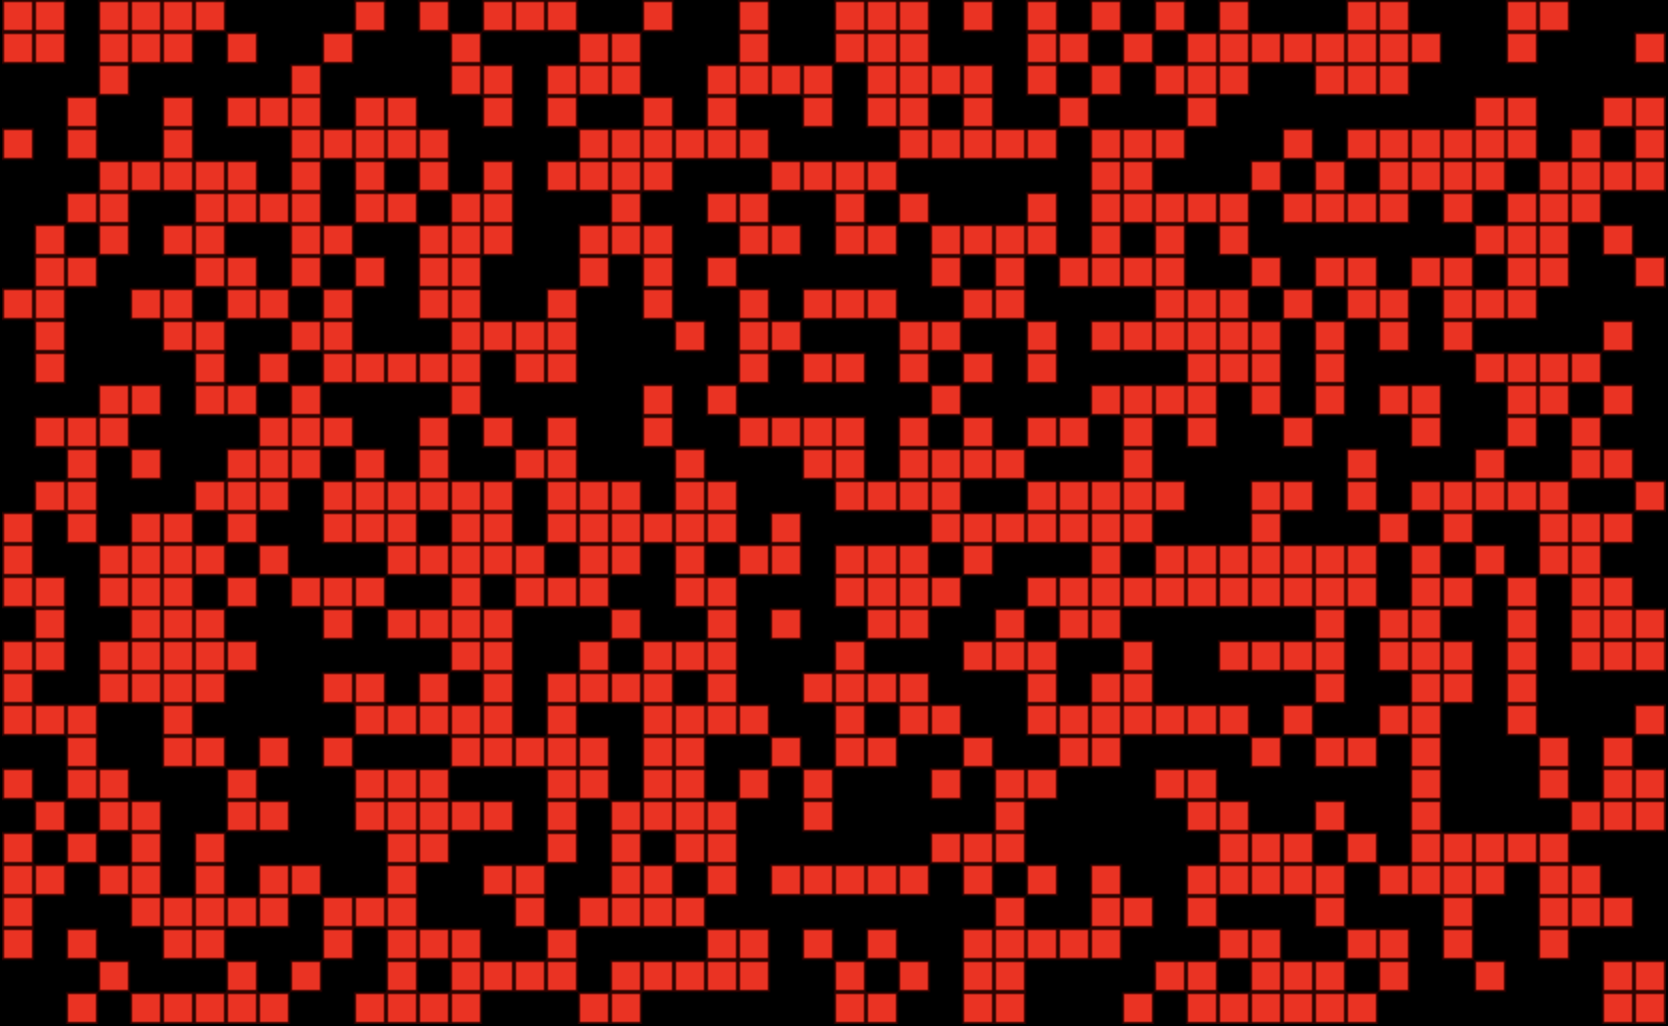
\includegraphics[width=\textwidth]{initial-cave.png}
	\caption{The initial cave on a randomized board}
	\label{fig:initialCave}
\end{figure}

\begin{figure}[h]
	\centering
	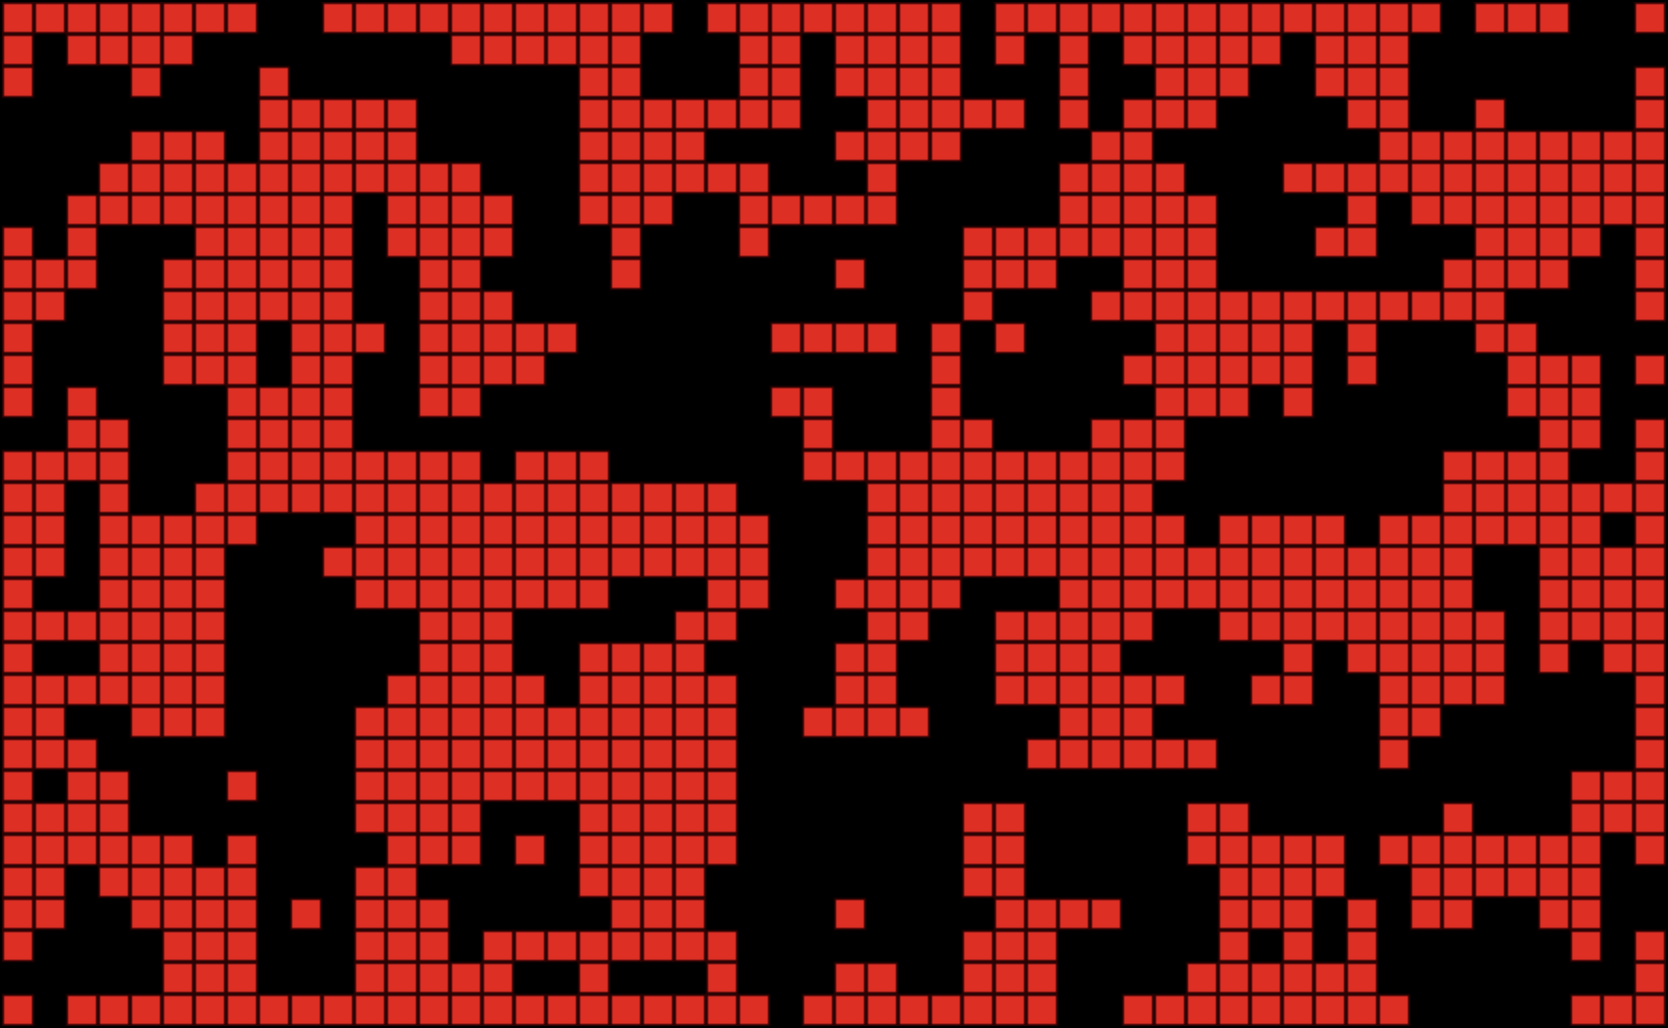
\includegraphics[width=\textwidth]{one-step-cave.png}
	\caption{The final cave after reaching a steady state}
	\label{fig:oneStepCave}
\end{figure}

\begin{figure}[h]
	\centering
	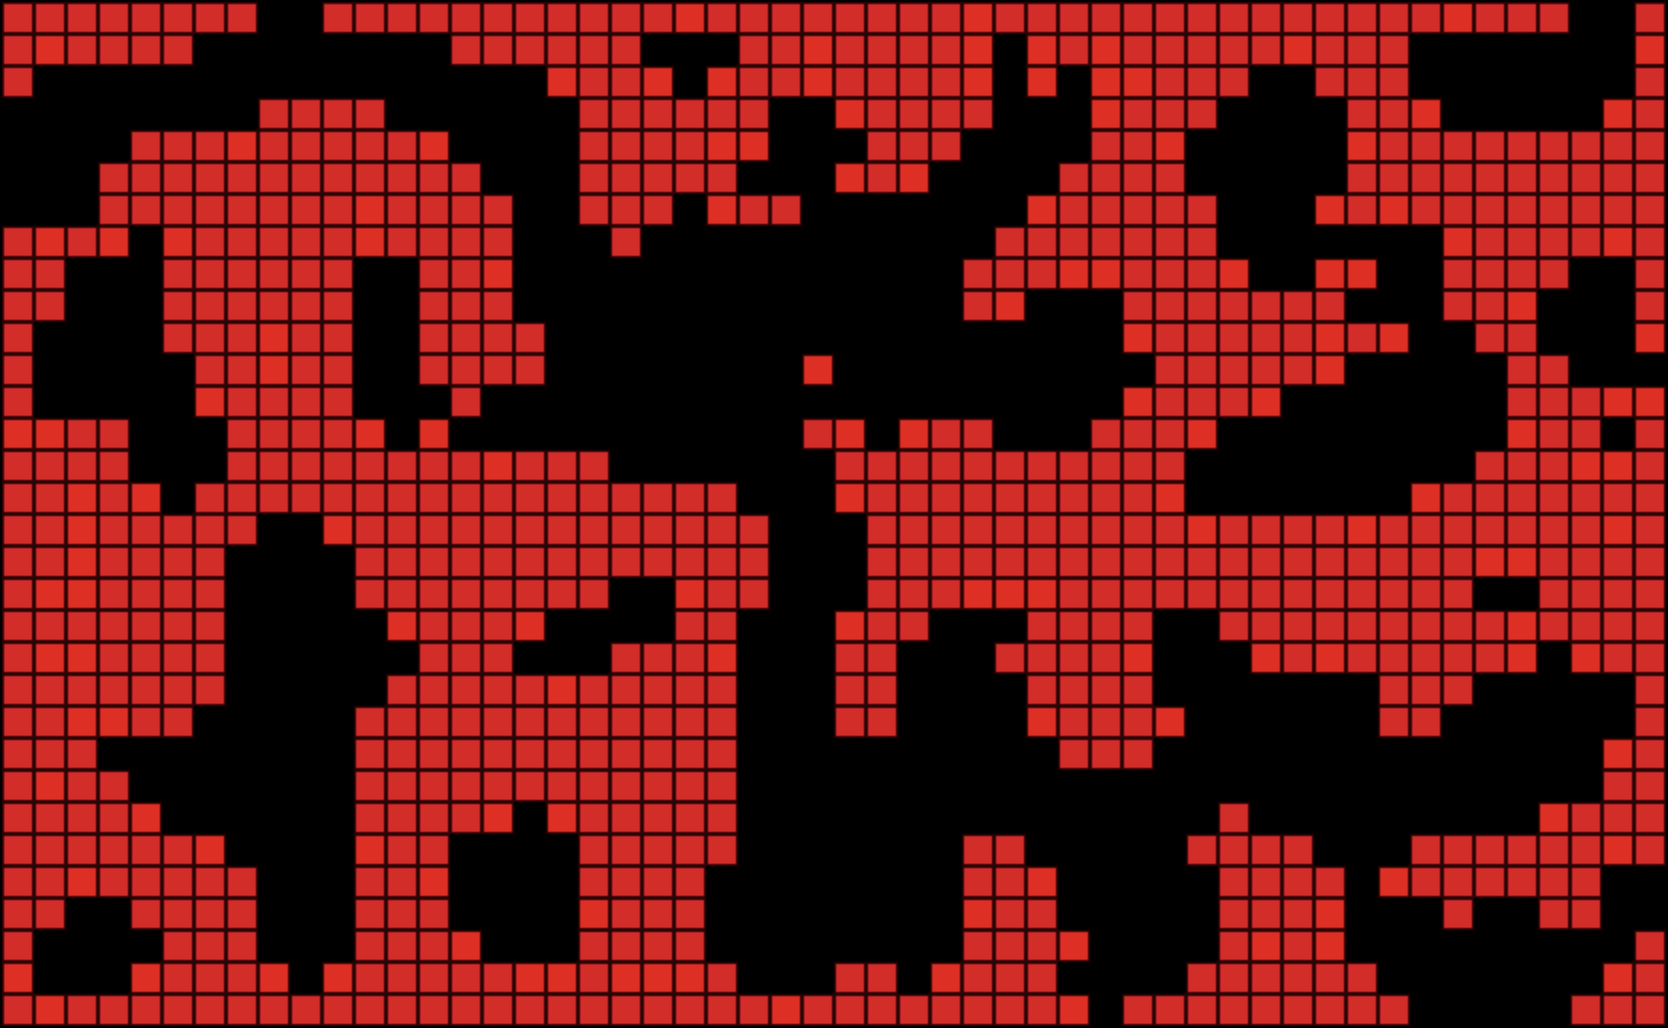
\includegraphics[width=\textwidth]{two-step-cave.png}
	\caption{The cave after two steps}
	\label{fig:twoStepCave}
\end{figure}

\begin{figure}[h]
	\centering
	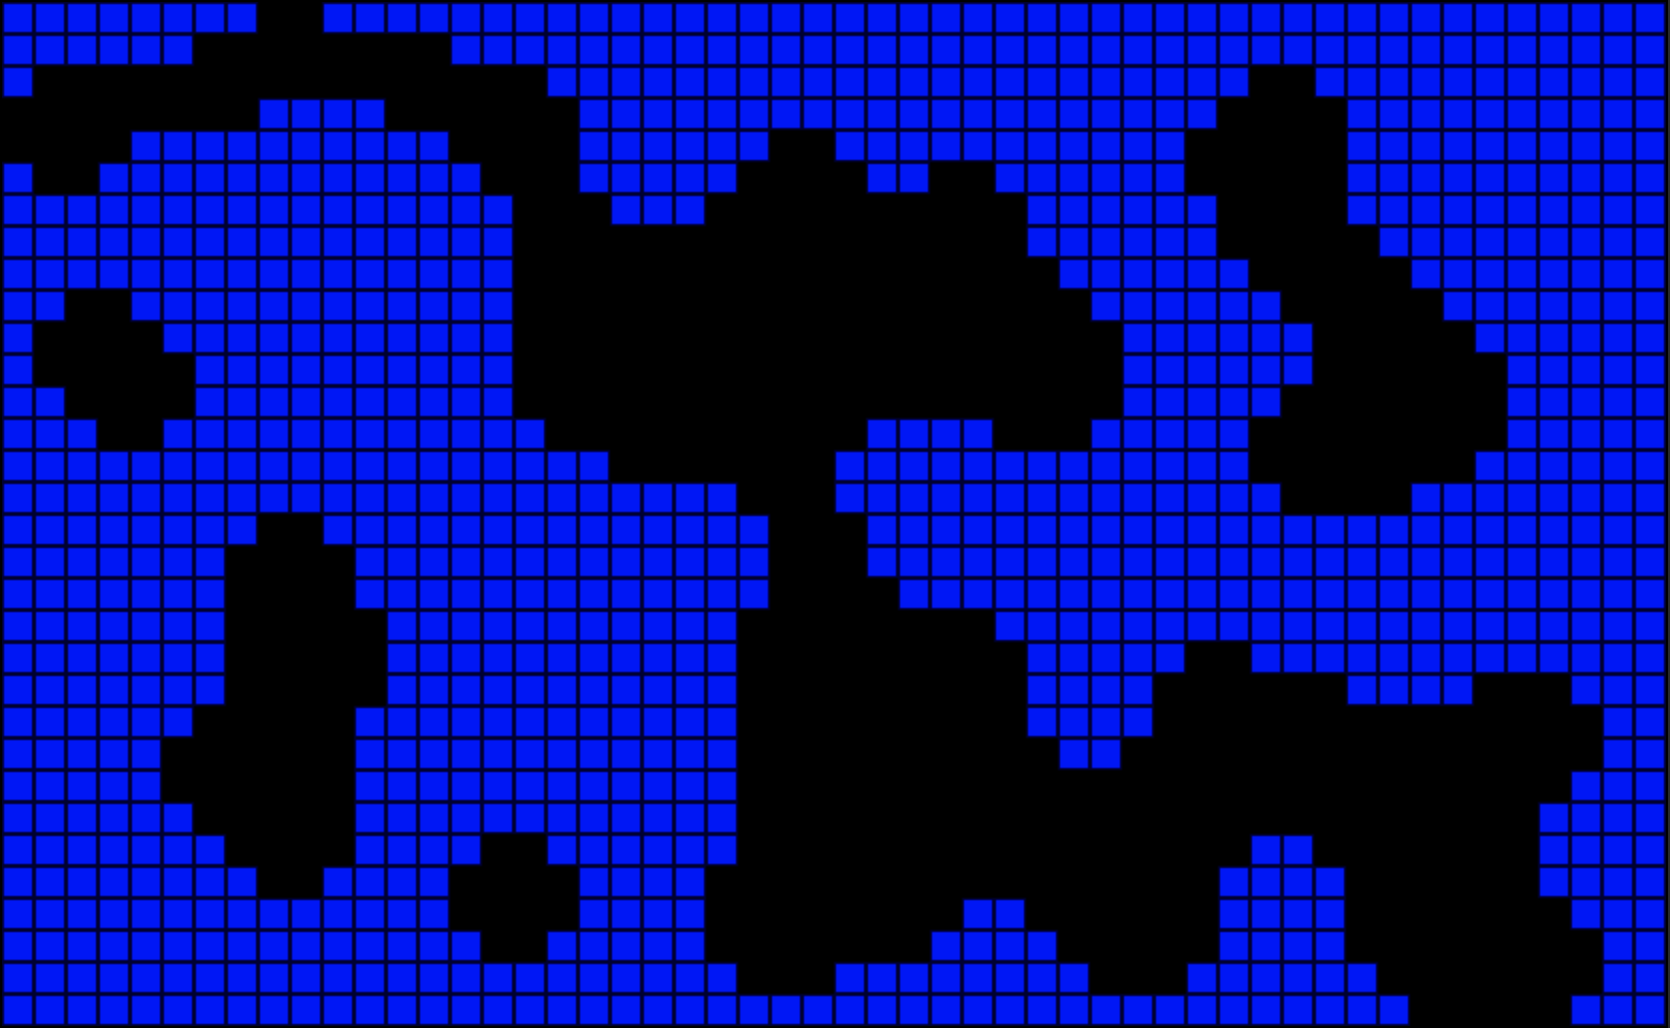
\includegraphics[width=\textwidth]{final-cave.png}
	\caption{The final cave after reaching a steady state}
	\label{fig:finalCave}
\end{figure}

\clearpage

\printbibliography

\end{document}

